\documentclass[../talk.tex]{subfiles}
\begin{document}

\begin{frame}{Regular separability}
    \begin{overlayarea}{\slidewidth}{\slideheight}


            \begin{problem}
                \problemtitle{Regular separability for \alert{class $\calF$}}
                \probleminput{Languages $\calL, \calK$ from class $\calF$.}
                \problemquestion{Is there $\calR$ \alert{regular} with $\calL \subseteq \calR$
                and $\calK \cap \calR = \emptyset$?}
            \end{problem}

        \vspace*{1em}


            $\calR$ is an \alert{abstraction} of $\calL$
            that is a \alert{certificate} for  $\calL \cap \calK = \emptyset$.

        \vspace*{1em}

            Only makes sense if $\calR$ is from a simpler class!

        \only<1>%
        {%
            \begin{center}
                \begin{tikzpicture}
                    \draw [semithick, opacity=0] (-1.5,-1.5) rectangle (3,1.5);
                    \draw [semithick,fill=tubsred!80!white] (-1.25,-1.25) rectangle (1.25,1.25);
                    \draw [semithick] (0,0) circle (1cm) node {$\calL$};
                    \draw [semithick] (2.5,0) circle (1cm) node {$\calK$};

                    \node at (-1,-1) {$\calR$};
                \end{tikzpicture}
            \end{center}
        }

        \only<2>%
        {%
            \begin{center}
                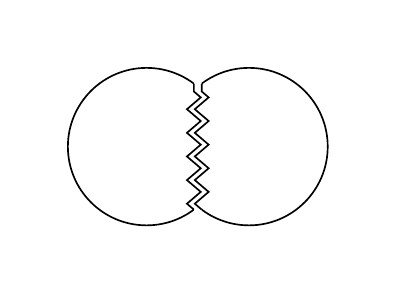
\begin{tikzpicture}
                    \draw [semithick, opacity=0] (-1.5,-1.5) rectangle (3,1.5);
                    \begin{scope}
                    \clip (-1.5,-1.5) rectangle (0.6,1.5);
                    \draw [semithick] (0,0) circle(1cm) node [xshift=-0.2cm]{$\calL$};
                    \end{scope}
                    \draw [semithick,decorate, decoration={zigzag, segment length=3mm}] (0.6,-0.8) -- (0.6,0.8);
                    \begin{scope}
                    \clip (0.7,-1.5) rectangle (3,1.5);
                    \draw [semithick] (1.3,0) circle(1cm) node [xshift=0.2cm] {$\calK$};
                    \end{scope}
                    \draw [semithick,decorate, decoration={zigzag, segment length=3mm}] (0.7,-0.8) -- (0.7,0.8);
                \end{tikzpicture}

                    No \alert{separator} exists!
            \end{center}

        }
        \only<3>%
        {%
            \begin{center}
                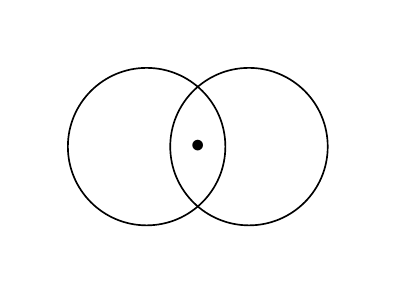
\begin{tikzpicture}
                    \draw [semithick, opacity=0] (-1.5,-1.5) rectangle (3,1.5);
                    % \begin{scope}                       % start of clip scope
                    % \clip (0,0) circle (1cm);
                    % \fill[orange] (1.5,0) circle (1cm);
                    % \end{scope}                         % end of clip scope
                    \draw [semithick] (0,0) circle (1cm) node {$\calL$};
                    \draw [semithick] (1.3,0) circle (1cm) node {$\calK$};
                    \node  at (0.65,0) {\alert{$\bullet$}};
                \end{tikzpicture}

                No \alert{separator} exists!
            \end{center}


        }

    \end{overlayarea}
\end{frame}

\end{document}
